\def\year{2020}\relax
%File: formatting-instruction.tex
\documentclass[letterpaper]{article} % DO NOT CHANGE THIS
\usepackage{aaai20}  % DO NOT CHANGE THIS
\usepackage{times}  % DO NOT CHANGE THIS
\usepackage{helvet} % DO NOT CHANGE THIS
\usepackage{courier}  % DO NOT CHANGE THIS
\usepackage[hyphens]{url}  % DO NOT CHANGE THIS
\usepackage{graphicx} % DO NOT CHANGE THIS
\urlstyle{rm} % DO NOT CHANGE THIS
\def\UrlFont{\rm}  % DO NOT CHANGE THIS
\usepackage{graphicx}  % DO NOT CHANGE THIS
\frenchspacing  % DO NOT CHANGE THIS
\setlength{\pdfpagewidth}{8.5in}  % DO NOT CHANGE THIS
\setlength{\pdfpageheight}{11in}  % DO NOT CHANGE THIS

\usepackage{amsthm}
\usepackage{mathtools}
\usepackage{tikz}
\usetikzlibrary{positioning}
\usepackage{algorithm}
\usepackage{algpseudocode}
\usepackage{algorithmicx}

\newcommand{\citename}[1]{\citeauthor{#1}, (\citeyear{#1})}

\DeclarePairedDelimiter\ceil{\lceil}{\rceil}
\DeclarePairedDelimiter\floor{\lfloor}{\rfloor}
\newcommand{\tup}[1]{\langle #1 \rangle}
\renewcommand{\cal}[1]{\mathcal{#1}}
\newcommand{\R}{\mathbb{R}}
\newcommand{\eps}{\varepsilon}
\newcommand{\Ch}{\mathit{Ch}}
\newcommand{\ch}{\mathit{ch}}
\newcommand{\CC}{\mathit{CC}}
\newcommand{\SCC}{\mathit{SCC}}
\newcommand{\core}{\mathit{Core}}
\newcommand{\samples}{\omega}


\newtheorem{theorem}{Theorem}[section]
\newtheorem{proposition}[theorem]{Proposition}
\newtheorem{lemma}[theorem]{Lemma}
\theoremstyle{definition}
\newtheorem{example}[theorem]{Example}
\newtheorem{definition}[theorem]{Definition}

\usepackage{multirow}
%\nocopyright
%PDF Info Is REQUIRED.
% For /Author, add all authors within the parentheses, separated by commas. No accents or commands.
% For /Title, add Title in Mixed Case. No accents or commands. Retain the parentheses.
 \pdfinfo{
/Title (Learning Cooperative Solution Concepts From Voting Behavior: a Case Study on the Israeli Parliament)
% /Author (Wei Lu, Alan Tsang, Yair Zick)
/Author (Anonymous)
/Keywords (Game Theory)
} %Leave this	
% /Title ()
% Put your actual complete title (no codes, scripts, shortcuts, or LaTeX commands) within the parentheses in mixed case
% Leave the space between \Title and the beginning parenthesis alone
% /Author ()
% Put your actual complete list of authors (no codes, scripts, shortcuts, or LaTeX commands) within the parentheses in mixed case. 
% Each author should be only by a comma. If the name contains accents, remove them. If there are any LaTeX commands, 
% remove them. 

% DISALLOWED PACKAGES
% \usepackage{authblk} -- This package is specifically forbidden
% \usepackage{balance} -- This package is specifically forbidden
% \usepackage{caption} -- This package is specifically forbidden
% \usepackage{color (if used in text)
% \usepackage{CJK} -- This package is specifically forbidden
% \usepackage{float} -- This package is specifically forbidden
% \usepackage{flushend} -- This package is specifically forbidden
% \usepackage{fontenc} -- This package is specifically forbidden
% \usepackage{fullpage} -- This package is specifically forbidden
% \usepackage{geometry} -- This package is specifically forbidden
% \usepackage{grffile} -- This package is specifically forbidden
% \usepackage{hyperref} -- This package is specifically forbidden
% \usepackage{navigator} -- This package is specifically forbidden
% (or any other package that embeds links such as navigator or hyperref)
% \indentfirst} -- This package is specifically forbidden
% \layout} -- This package is specifically forbidden
% \multicol} -- This package is specifically forbidden
% \nameref} -- This package is specifically forbidden
% \natbib} -- This package is specifically forbidden -- use the following workaround:
% \usepackage{savetrees} -- This package is specifically forbidden
% \usepackage{setspace} -- This package is specifically forbidden
% \usepackage{stfloats} -- This package is specifically forbidden
% \usepackage{tabu} -- This package is specifically forbidden
% \usepackage{titlesec} -- This package is specifically forbidden
% \usepackage{tocbibind} -- This package is specifically forbidden
% \usepackage{ulem} -- This package is specifically forbidden
% \usepackage{wrapfig} -- This package is specifically forbidden
% DISALLOWED COMMANDS
% \nocopyright -- Your paper will not be published if you use this command
% \addtolength -- This command may not be used
% \balance -- This command may not be used
% \baselinestretch -- Your paper will not be published if you use this command
% \clearpage -- No page breaks of any kind may be used for the final version of your paper
% \columnsep -- This command may not be used
% \newpage -- No page breaks of any kind may be used for the final version of your paper
% \pagebreak -- No page breaks of any kind may be used for the final version of your paperr
% \pagestyle -- This command may not be used
% \tiny -- This is not an acceptable font size.
% \vspace{- -- No negative value may be used in proximity of a caption, figure, table, section, subsection, subsubsection, or reference
% \vskip{- -- No negative value may be used to alter spacing above or below a caption, figure, table, section, subsection, subsubsection, or reference

\setcounter{secnumdepth}{2} %May be changed to 1 or 2 if section numbers are desired.

% The file aaai20.sty is the style file for AAAI Press 
% proceedings, working notes, and technical reports.
%
\setlength\titlebox{2.5in} % If your paper contains an overfull \vbox too high warning at the beginning of the document, use this
% command to correct it. You may not alter the value below 2.5 in
\title{Learning Cooperative Solution Concepts From Voting Behavior:\\ A Case Study on the Israeli Parliament}
%Your title must be in mixed case, not sentence case. 
% That means all verbs (including short verbs like be, is, using,and go), 
% nouns, adverbs, adjectives should be capitalized, including both words in hyphenated terms, while
% articles, conjunctions, and prepositions are lower case unless they
% directly follow a colon or long dash
% \author{Wei Lu\\
% School of Computing\\
% National University of Singapore\\
% weilu@u.nus.edu
% \And
% Alan Tsang\\
% School of Computing\\
% National University of Singapore\\
% akhtsang@nus.edu.sg
% \And
% Yair Zick\\
% School of Computing\\
% National University of Singapore\\
% dcsyaz@nus.edu.sg
% }
\author{Paper 4675}
 \begin{document}

\maketitle

\begin{abstract}
Most frameworks for computing solution concepts in hedonic games are theoretical in nature, and assume complete knowledge of all agent preferences which is impractical in real world settings.
Recent work introduces the theoretical foundation of Probably Approximately Correct (PAC) stability to model stability under uncertainty through sampling.
In this paper, we present the first application of strategic hedonic game models on real-world data.
We provide an algorithmic improvement for discovering PAC stable solutions, which we apply on voting data from the Israeli parliament (Knesset). 
We discover that PAC stable solutions under top responsive preferences reflect Knesset members' political positions at large, when compared against ground truth party affiliations.
Moreover, these comparisons also reveal politicians whose voting behaviors are known to deviate from party lines.
Finally, we show that PAC hedonic game models compare favorably to both $k$-means clustering and stochastic block models, which do not account for strategic behavior, for uncovering voting patterns.
\end{abstract}

\section{Introduction}\label{sec:intro}
Cluster analysis is an essential task of exploratory data mining. It has been studied extensively by the machine learning community. However, most works that took the data driven approach completely ignore an individual player's utility and their strategic behaviors. Meanwhile in the field of game theory, the computational social choice community puts in considerable efforts studying stability related solution concepts of coalition formation games with hedonic preferences; however most works are purely theoretical. In addition, existing stable solution finding algorithms require full visibility of all agents' preferences, which is a major obstacle in applying the research on real-world collaborative activities.

Recent research by \citename{ijcai2017-380} lays down the theoretical foundation of Probably Approximately Correct (PAC) stability; they provide an algorithm which produces a partition that is likely resistant to deviation given limited knowledge of agents' hedonic preferences as input. This opens the possibility of constructing models taking the data driven approach, at the same time accounts for agents' strategic behaviors.

In this paper, we present the first application of strategic hedonic games models on real-world data. We answer the following research questions: Can we use hedonic games to model real-world collaborative activities? How well does the outcome compare to ground truth? How well does the outcome compare to that of canonical clustering and community detection models'?

\subsection{Our Contributions}\label{sec:contrib}
Our contribution includes an algorithmic improvement for finding a PAC stable solution for top responsive games --- a sub-class of hedonic games (Section~\ref{sec:improved_algo}). We take the Israeli parliament (the Knesset) members' past voting records on legislative bills (Section~\ref{subsec:data}), construct top responsive preference models, and apply the improved algorithm to produce PAC stable partitions (Section~\ref{subsec:exp_pac_models}). We detail in our analysis (Section~\ref{subsec:exp_analysis}), by using the party affiliations as the ground truth partition, our PAC partitions are able to reveal the Knesset members' political positions at large. Comparing to $k$-means clustering and stochastic block models (Section~\ref{subsec:exp_comparison_models}), one of our PAC models reveals politicians whose voting behaviors are known to break from their party affiliations and whose allegiance is fickle.

\subsection{Related Work}\label{sec:related}
Past works on hedonic preferences focus on the existence and computational aspect of stability concepts in various sub-classes of hedonic coalition formation games \cite{Aziz:2012:ESH:2343776.2343806}, \cite{aziz_savani_moulin_2016}. The specific subclass we are interested in is top responsive games, which captures the idea that a player's utility is derived from the most preferred set of other players in her coalition.
\citename{ALCALDE2004869} show that top responsive games guarantee the existence of a core stable partition, which is discoverable through the Top Covering Algorithm. \citename{DIMITROV2007130} simplify the original Top Covering Algorithm and proved that it not only constructs a core, but a strict core. \citename{Dimitrov2006TopRA} also show that adding the mutuality condition the simplified top covering algorithm produces a Nash stable partition. \citename{Aziz:2012:ESH:2343776.2343806} further prove that with mutuality the partition produced is in fact strict strong Nash stable for any top responsive game. We formulate our empirical experiments upon recent work by \citename{ijcai2017-380} on PAC stability. We will discuss the technical details of top responsive games, various stability concepts, mutuality, relevant algorithms, and PAC stability in Section~\ref{sec:prelim}.

\section{Preliminaries}\label{sec:prelim}
A {\it hedonic game} is a pair $(N, P)$, where $N$ is a finite set of players $\{1, \cdots, n\}$ and $P$ is a {\it preference profile} consisting of preference relations $\succeq_i$ for every player $i \in N$: $P = (\succeq_1, \cdots, \succeq_n)$. A {\it preference relation} $\succeq_i$ is a reflective, complete, and transitive binary relation on $\mathcal{N}_i$, where $\mathcal{N}_i$ is the set of all non-empty subset of $N$ that includes player $i$; i.e., $\mathcal{N}_i = \{S \subseteq N: i \in S, S \neq \emptyset \}$

Consider a parliament; who are "natural allies"? One way to model this is by assuming that each member has a preference relation over various groups they wish to be part of; our objective is to identify partitions (also known as {\it coalition structures}) that satisfy certain desirable properties, such as stability.

\subsection{Hedonic Preference Models}
We are learning preferences from data, but still need to make certain assumptions about a player's utility model. We now describe the two preference models our study is built upon.

\paragraph{Top Responsive Preferences}
The intuition behind top responsiveness is that every player derives their utility from the most preferred subset players of the coalition they belong. If two coalitions, with one containing the other, yield the same utility for a player, the tie is broken in favor of the smaller coalition. 

A player $i$'s most preferred sets of coalitions is called {\it choice sets}: $\Ch(i, S) = \{S' \subseteq S: (i \in S') \wedge (S' \succeq_i S'' \forall S'' \subseteq S)\}$. The unique choice set in $\Ch(i, S)$ is denoted as $\ch(i, S)$. A {\em top responsive} preference profile requires that for any player $i \in N$, and any coalition that may contain player $i$: $S, T \in \mathcal{N}_i$:
\begin{enumerate}
  \item $|\Ch(i, S)| = 1$.
  \item if $\ch(i, S) \succ_i \ch(i, T)$ then $S \succ_i T$
  \item if $\ch(i, S) = \ch(i, T)$ and $S \subset T$ then $S \succ_i T$
\end{enumerate}

\paragraph{Appreciation of Friends Preferences}
The description of a generic top responsive preference profile is exponentially large in the number of players, as each player needs to rank all possible coalitions they may belong to, therefore we turn our attention to a sub-class of top responsive preferences –-- appreciation of friends preferences.

In this preference model, a player classifies other players as either friends or enemies, and prefers any coalition with more friends and fewer enemies: Let $G_i$ be player $i$'s set of friends, and $B_i$ the set of enemies. $G_i \cup B_i \cup i = N$ and $G_i \cap B_i = \emptyset$. A preference profile $P^f$ is based on {\it appreciation of friends} if for all player $i \in N$, $S \succeq_i T$ if and only if $|S \cap G_i| > |T \cap G_i|$ or $|S \cap G_i| = |T \cap G_i|$ and $|S \cap B_i| \leq |T \cap B_i|$.

\subsection{Stability Concepts} \label{subsec:stability}
We are particularly interested in models that produce partitions that satisfy strategic considerations; specifically, we focus our attention on stability concepts that capture the idea that no group of players can be better off by leaving and forming their own coalition. Group based stability notions are stronger than those based on individual deviation, such as Nash stability, because individual based stability concepts do not account for the disutility of the group an individual player is joining or leaving.

\paragraph{Core \& Strict Core}
A coalition $S \subseteq N$ {\it strongly blocks} a coalition structure $\pi$ if every player $i \in S$ strictly prefers $S$ over its current coalition $\pi(i)$; a coalition structure $\pi$ is {\it core stable} when there is no strongly blocking coalition $S$. 
A coalition $S \subseteq N$ {\it weakly blocks} a coalition structure $\pi$ if every player $i \in S$ weakly prefers $S$ over its current coalition $\pi(i)$ and there exists at least one player $j \in S$ who strictly prefers $S$ over $\pi(j)$; a coalition structure is strictly core stable when there is no weakly blocking coalition.

\paragraph{Strong Nash \& Strict Strong Nash}
Next we cover two solution concepts with even stronger notions of stability based on group deviation. 
If a partition $\pi' \neq \pi$ exists with movement of players $S \subseteq N$ and $S \neq \emptyset$ (denoted as $\pi \xrightarrow{S} \pi'$), where $\forall i \in S$, $\pi'(i) \succ_i \pi(i)$, and $\forall j \in N\text{\textbackslash}S$, $\pi'(j) = \pi(j)$, then $S$ strongly Nash blocks $\pi$. 
A partition that admits no strongly Nash blocking set $S \subseteq N$ is said to be strong Nash stable (SNS). A non-empty set of players $S \subseteq N$ weakly Nash blocks $\pi$ if $\forall i \in S$, $\pi'(i) \succeq_i \pi(i)$ and $\exists j \in S$, $\pi'(j) \succ_j \pi(j)$. 
A partition that admits no weakly Nash blocking set $S \subseteq N$ is said to be strict strong Nash stable (SSNS).

\paragraph{} 
A top responsive preference profile guarantees the existence of a strict core partition. Moreover, top responsiveness also warrants a strict strong Nash stable partition if all players preference relations are {\it mutual} ––– for all $i, j \in N$, for all coalition that contains $i$ and $j$: $S \in \mathcal{N}_i \cap \mathcal{N}_j$, $i \in ch(j, S)$ if and only if $j \in ch(i, S)$. This means if we can model empirical data with mutual preferences, we can achieve the strongest notion of group based notion of stability.

\subsection{Complete Preference Profile Algorithms} \label{subsec:full_pref_algos}
The top covering algorithm computes a strict core stable partition for top responsive games.

\begin{algorithm}[htb]
  \caption{Top Covering Algorithm}
  \label{alg:top_covering}
  \textbf{Input:} A hedonic game satisfying top responsiveness.

  \begin{algorithmic}[1]
  \State $R^1 \leftarrow N$; $\pi \leftarrow \emptyset$.

  \For{$k=1$ to $|N|$}
    \State \label{top_cover:select} Select $S^k$
    \State \label{top_cover:remove} $\pi \leftarrow \pi \cup \lbrace S^k \rbrace$ and $R^{k+1} \leftarrow  R^k \setminus S^k$
    \If {$R^{k+1} = \emptyset$}
      \State \Return $\pi$
    \EndIf
  \EndFor

  \State \Return $\pi$
 \end{algorithmic}
\end{algorithm}

Let $\CC(i, S)$ denotes the connected component with $i$ as the root node,
in the graph induced by $S$ as vertices and directed edges $E$,
$(i, j) \in E$ if $j \in \ch(i, S)$ for all $j \in S$.
Step~\ref{top_cover:select} then expands to the following: select $i\in R^k$ such that $|\CC(i,R^k)| \leq |\CC(j,R^k)|$ for each $j\in R^k$; and $S^k\leftarrow \CC(i,R^k)$

Note that the input of the top covering algorithm is the entire preference profile of all players, which is in the order of $O(2^{|N|})$. Finding the choice set for every player after each round of player removal at Step~\ref{top_cover:remove} requires scanning through every remaining player's preference relation, which makes the most expensive part of this algorithm, so this algorithm is exponential time in the number of players.

\citename{Dimitrov2006} propose a similar algorithm for finding a strict core stable coalition structure in polynomial time in the number of players specifically for appreciation-of-friends preference profiles. Their algorithm effectively replaces Step~\ref{top_cover:select} of Algorithm~\ref{alg:top_covering} with finding the largest strongly connected component (SCC) in the graph induced by $R^k$. Due to the definition of appreciation of friends preference profile, Step~\ref{top_cover:remove} no longer requires scanning through every remaining player's preference relation for removed players, making the partition equivalently the strongly connected components of the graph induced by $N$.

\subsection{PAC Learning and PAC Stability}
Probably Approximately Correct (PAC) learning is the canonical framework for provable probabilistic approximations to functions. In this framework, a learner receives samples and selects a function from a class of possible functions. The selected function is called the {\it hypothesis}, which should be likely to predict new samples from the same distribution. A good probabilistic approximation means that with probability of at least $1 - \delta$, the selected function's output has an average error less than or equal to $\varepsilon$, where $0 < \varepsilon, \delta < 1$. A hypothesis class is efficiently PAC learnable if such a good probabilistic approximation can be produced by some algorithm that has both running time and input sample size be polynomial in $n$, $\frac{1}{\varepsilon}$, and $\log{\frac{1}{\delta}}$.

\citename{ijcai2017-380} define that a class of hedonic games is PAC stablizable if there exists an algorithm that produces a partition $\pi$ such that $\Pr_{S\sim D}[\text{S core blocks } \pi] < \varepsilon$; both the number of samples required by the algorithm to provide this PAC guarantee, and the running time of producing a consistent solution are polynomial in $n$, $\frac{1}{\varepsilon}$, and $\log{\frac{1}{\delta}}$. In the same paper, \citename{ijcai2017-380} also showed that top responsive games are efficiently PAC stablizable even though they are not PAC learnable. The PAC stable partition can be computed with Algorithm~\ref{alg:pac_top_covering}.

\begin{algorithm}[htb]
  \caption{PAC Top Covering Algorithm}
  \label{alg:pac_top_covering}
  \textbf{Input:} $\eps$, $\delta$, set $\cal S$ of $m = (2n^4 + 2n^3)\ceil{\frac{1}{\eps}\log\frac{2n^3}{\delta}}$ samples from $\cal D$
  \begin{algorithmic}[1]

  \State $R^1 \gets N$, $\pi \gets \emptyset$
  \State $\samples \gets \ceil{2n^2 \frac{1}{\eps}\log\frac{2n^3}{\delta}}$
  \For{$k=1$ to $|N|$}

    \State \label{pac_top_cover:sample_begin} $\cal S' \gets$ take and remove $\samples$ samples from $\cal S$
    \State $\cal S' \gets \{T: T \in \cal S', T \subseteq R^k\}$
    \For{$i \in R^k$}
      \If{$i \notin \bigcup_{X \in \cal S'} X$}
        \State$B_{i,k} \gets \{i\}$
      \Else
        \State $B_{i,k} \in \arg\max_{T \in \cal S'}{v_i(T)}$
        \State $B_{i,k} \gets \underset{\{T \in \cal S' : \ch(i,T) = \ch(i,B_{i,k})\}}{\bigcap} T$.
      \EndIf
    \EndFor

    \For{$j = 1,\dots,|R^k|$}
      \State $\cal S'' \gets$ take and remove $\samples$ samples from $\cal S$
      \State $\cal S'' \gets \{T: T \in \cal S'', T \subseteq R^k\}$
      \For{$i \in R^k$}
        \State $B_{i,k} \gets B_{i,k} \cap \underset{T \in \cal S'' : \ch(i,T) = \ch(i,B_{i,k})}{\bigcap} T$.
      \EndFor
    \EndFor \label{pac_top_cover:sample_end}

    \State Select $i\in R^k$ such that $|\CC(i,R^k)| \leq |\CC(j,R^k)|$ for each $j\in R^k$.
    \State $S^k\leftarrow  \CC(i,R^k)$; $\pi \leftarrow  \pi \cup \lbrace S^k \rbrace$;  and $R^{k+1} \leftarrow  R^k \setminus S^k$
    \If {$R^{k+1} = \emptyset$}
      \State \Return $\pi$
    \EndIf
  \EndFor

  \State \Return $\pi$
 \end{algorithmic}
\end{algorithm}

In Algorithm~\ref{alg:pac_top_covering}, every sample $j$ consists of a coalition $S_j \subseteq N$, and the values assigned to $S_j$ by each of its member $\vec{v}(S_j) = (v_i(S_j))_{i \in S_j}$.

\section{Improved PAC Top Covering Algorithm}\label{sec:improved_algo}
We discover that we can make the PAC top covering algorithm more efficient by replacing the step of finding the smallest $\CC$ with finding the largest Strongly Connected Component ($\SCC$). Our algorithmic improvement is based on \citename{Dimitrov2006}'s appreciation-of-friends strict core partition discovery algorithm. We first show that the appreciation-of-friends algorithm generalizes to all top responsive games; then we demonstrate that making the same modification to the PAC top covering algorithm still produces a PAC stable partition but with improved running time complexity.

\begin{proposition}
\label{prop:scc_generalizes}
  The appreciation-of-friends algorithm produces a strictly core stable partition given any top responsive preference profile.
\end{proposition}

\begin{proof}
Assuming the resulting partition of the $SCC$ procedure $\pi$ is not strictly core stable, then there exists at least one weakly blocking coalition $S \subseteq N$ and at least one player $i \in S$ prefers $S$ over $\pi(i)$. Consider the step when the coalition $\pi(i)$ is generated --- it was the largest strongly connected component in the directed graph induced by remaining players' choice sets. In order to form $S$ which is different from $\pi(i)$, either or both of the following steps must be carried out:

\begin{enumerate}
  \item at least one player $j \in \pi(i)$ needs to be removed from $\pi(i)$
  \item at least one player $k \notin \pi(i)$ needs to be added to $\pi(i)$
\end{enumerate}

When only Step 1 is carried out, since $\pi(i)$ is a strongly connected component, $j$ has at least one incoming edge, which means it is in the choice set of at least one other player $j' \in \pi(i)$, therefore its removal makes player $j' \in S$ worse off, therefore $S$ cannot be weakly blocking $\pi$.

When only Step 2 is carried out, since player $k$ was not part of the strongly connected component that induces $\pi(i)$, $k$ only has incoming or outgoing edges between itself and the $\SCC$ but not both. If $k$ only has outgoing edges to $\SCC$ it means adding $k$ to $\pi(i)$ will only make $k$ better off, but other players in $\pi(i)$ worse off because $S = \pi(i) \cup \{k\}$ is bigger in size $|S| > |\pi(i)|$ while for any player $i' \in S, i' \neq k$ their choice set remains the same, therefore making $S$ less preferable than $\pi(i)$ for player $i' \in S, i' \neq k$ per definition of top responsiveness. Therefore $S$ is not blocking $\pi$ when $k$ only has outgoing edges to $\SCC$. In the case $k$ only has incoming edges from $\SCC$, it means adding $k$ to $\pi(i)$ will only make some player $i \in \pi(i)$ better off as $k$ is in their choice set. 
However $k$ will be made worse off by this move, since none of the player in $\pi(i)$ is in $k$'s choice set. As such, $S$ is not blocking $\pi$ when only Step 2 is carried out.

When both Step 1 and Step 2 are carried out to form $S$ from $\pi(i)$, since Step 1 is bound to make some player $j' \in \pi(i)$ worse off, the only way to compensate $j'$ is by adding someone from their choice set to $\pi(i)$. Assuming $k$ is in $j'$'s choice set, then $k$ only has incoming edges from the $\SCC$, which means $k$ will be worse off by joining $\pi(i)$, so $S$ cannot be blocking $\pi$.
\end{proof}

\begin{theorem}
  The $\SCC$ based PAC algorithm produces a PAC stable partition given a top responsive preference profile.
\end{theorem}

\begin{proof}[Proof Sketch]
\citename{ijcai2017-380} already prove that their PAC algorithm efficiently PAC stabilizes top responsive games. 
The correctness of their PAC algorithm relies on the fact that the coalition selection and deletion procedure based on finding the smallest $\CC$ produces a core stable partition when there's full visibility to players' choice sets; the PAC guarantee is an artefact of choice set approximation through sampling (Algorithm~\ref{alg:pac_top_covering} Step~\ref{pac_top_cover:sample_begin} to Step~\ref{pac_top_cover:sample_end}). 
Our modification to their algorithm does not change how players' choice sets are approximated; we only modified how coalitions are selected. 
We show in Proposition~\ref{prop:scc_generalizes} that modifying the coalition selection procedure from $\CC$ to $\SCC$ still produces a strict core stable partition for top responsive games, therefore the $\SCC$ based PAC algorithm still produces a PAC stable partition.
\end{proof}

The largest $\SCC$ procedure provides a running time improvement over the smallest $\CC$ procedure because finding the smallest $\CC$ requires $\mathcal{O}(|V|(|V| + |E|))$ time while the largest $\SCC$ can be found using Tarjan's algorithm in linear time $\mathcal{O}(|V| + |E|)$\cite{Tarjan72depthfirst}. 
This running time improvement is only meaningful for the PAC version of the top covering algorithm due to the input size of the original top covering algorithm being exponential in the number of players. 
In addition, taking out more players in the earlier iterations also reduces the amount of computation required for the later iterations, making our experiments run much faster than what it would have been with the original $\CC$ procedure.

\section{Experiments} \label{sec:experiment}
Now we delve into the empirical experiments part of our study. First we present the dataset used and explain why it is a good choice for studying the efficacy of hedonic games in real-world settings. We then formulate two hedonic game models; we apply the improved PAC partition discovery algorithm described in Section~\ref{sec:improved_algo} to our dataset under the two assumed hedonic preference models. In addition, we describe two clustering and community detection models we adopt for comparison. Lastly we conduct political analysis of our experiment results.

\subsection{Data} \label{subsec:data}
The Israeli political system, in thanks, partially, to its use of proportional representation, is made of multiple parties. The Israeli Knesset is the national legislative branch of the Israeli government. We limit our study to the 20th Knesset (2015-2019), which is the last Knesset preceding the current one. In this Knesset there are 10 parties, but some parties are unions of smaller parties. In some cases the parties have merged (e.g., the Likud or Meretz), and in some cases, they have different organizational structure (e.g., the Jewish Home party or the Joint List).

While in the past, this preponderance of parties led to a multi-dimensional party system, leading to unexpected coalitions and combinations, in the past few decades Israeli parties can be, in general, ordered along a single right-left axis, which has to do mainly with the parties' approach to the Israeli-Palestinian conflict. This simplifies the considerations we need to take into account when analyzing the outcomes, and allows for easier comparison between the different models.  More over, it allows us to more easily discern unexpected coalition structures that need to be explained. There is also relative ideological cohesion between coalition parties as well as between opposition parties.

No Israeli party has ever been elected with a majority of Knesset seats, which means all governments are made of coalitions. In the past few years (including the Knesset we investigate) governments have tightened their grip over coalition parties by having a government committee issue a generally mandatory voting instructions for every proposed bill. The opposition, of course, is under no such control, but due to their relative ideologies, there is significant agreement.

The Knesset website provides data access through Open Data Protocol (OData) on all its parliament members, laws, and every member's votes on every law. The Kenesset has 120 seats, but the 20th Knesset has 147 parliament members due to some Knesset members resigning or joining mid-term.
We download all 147 parliament members' information including name, party affiliation and their votes for all 7515 bills deliberated. A vote can take on one of the following values 0 (vote canceled), 1 (vote for), 2 (vote against), 3 (abstained), 4 (did not attend). 

There were some inconsistencies found in the data, which we discovered by cross-checking against another dataset. With the help of the Knesset data team, we resolved the data inconsistency issue by removing votes for a small number of bills (26 in total) from the dataset.

\subsection{Top Responsive Game Model} \label{subsec:exp_pac_models}
Recall that top responsiveness models a preference profile where every player derives their utility for a given coalition based on only the most preferred subset of players in their coalition. In the context of our dataset, it captures the following idea: politicians care about whose votes they stand with; they want to vote with other politicians they like. Since we do not observe quantifiable preferences of each of the Knesset member over other members, we derive their preferences from the Knesset voting data assuming top responsiveness and mutuality. Top responsiveness guarantees a strictly core stable partition. With the addition of mutuality, as discussed in Section~\ref{subsec:stability}, a strict strong Nash stable partition can be computed using Algorithm ~\ref{alg:top_covering} if the full preference profile is given. When the complete preference profile is not available, we can use Algorithm ~\ref{alg:pac_top_covering} to approximate a strict strong Nash stable partition. We then compare the resulting partitions to party affiliations to assess the quality of our models.

\paragraph{Handcrafted Value Function}
First we attempt to formulate a generic top responsive preference model through representing every player's utility model using a value function. 
For each bill there are two natural coalitions: one formed by parliament members who voted ``for'', and the other formed by parliament members who voted ``against''. Note that the values assigned by members to their respective coalitions are not immediately well defined, so we define the player $i$'s value function for coalition $S$ as below:

\[
  v_i(S) = 
  \begin{dcases}
      1 + \frac{1}{|S|} + \frac{|S_p|}{|N|},& \text{if $S$ is the winning majority}\\
      0,              & \text{otherwise}
  \end{dcases}
\]

$S$ can take on one of the two values $\{S_f, S_a\}$, where $S_f$ is the set of members who voted ``for'' and $S_a$ is the set of members who voted ``against''. $S_p$ denotes the set of parliament members who participated $S_p = S_f \cup S_a$. $S_f$ is the winning majority if $|S_f| > |S_a|$, vice versa. When $|S_f| = |S_a|$, $S_a$ is considered to be the winning majority.

The conditional value function captures that a winning coalition, being successfully passing a bill or successfully blocking a bill, is always worth more than a losing coalition. $\frac{1}{|S|}$ reflects that a win is considered more valuable when it's achieved with fewer members, which is also conceptually consistent with top responsive game's preference for smaller coalitions. The partition term $\frac{|S_p|}{|N|}$ gives a win more value when more parliament members voted for or against the bill. For simplicity, we assume every member in a given coalition assigns equal value to their coalition.

This handcrafted value function allows us to construct a partial preference relation for every parliament member. We programmatically verified that this partial preference profile in fact does not satisfy top responsiveness. It makes this approach analogous to improper learning.

To simulate i.i.d, we sample $\frac{3}{4}$ of the bills with replacement. We repeated the algorithm run 50 times and observed that the resulting partition is consistent with little variability. It is not core stable with respect to the partial preference profile. This is unsurprising due to the PAC model. The partition has one large coalition consisting of around 60 members and the rest are all singleton coalitions. All members of the only large coalition are from right wing parties. The singleton coalitions are likely a result of the limited size of the derived partial preference profile --- Upon discovery of the smallest $\CC$ in each iteration, we also remove any coalition that contains any of the removed player from the remaining player's preference relation. Since we took away a large number of players in one of the first few iterations, many coalitions are removed from remaining players' preference relations, resulting in isolated nodes in the updated graph which leads to singleton coalitions. Despite the number of singleton coalitions, the largest coalition does reflect political position of about 40\% of the parliament members.

\begin{figure}[htb]
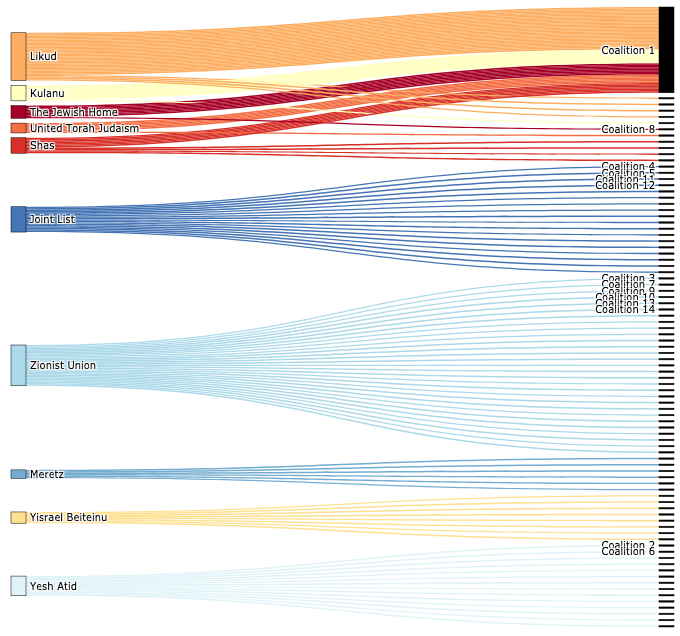
\includegraphics[width=\columnwidth]{pac_value_function}
\caption{Coalitions formed by the PAC model with the handcrafted value function, compared to party affiliations. Left wing parties are colored with blue hues, right wing red hues, center yellow hues.}
\end{figure}

\paragraph{Appreciation of Friends}
Our next set of experiments are based on the appreciation of friends model, which is a proper subset of top responsive games. We define friends of a player's as anyone whose votes agreed with the given player's more than disagreed. Agreed votes are only counted if the given player voted ``for'' or ``against''. We experimented with two different ways of counting the disagreed votes:

\begin{enumerate}
  \item Narrow disagreement: the other player's vote is different from mine, and is either ``for'' or ``against''
  \item Broad disagreement (selective friends): the other player's vote is different from mine
\end{enumerate}

Compared to narrow disagreement, broad disagreement leads to every player being more selective of friends. For any player, those who are not friends are considered enemies.

Note that as soon as the sets of friends and enemies are derived for each parliament member, we can expand them into a complete preference profile, and apply top covering algorithm to obtain a strict strong Nash stable partition with respect to the given preference profile. The broad disagreement setup produced a partition with 18 coalitions out of which there are two large coalitions with 66 and 58 members, respectively. One of these two large coalitions is made of left wing party politicians, while the other of right wing party members. In contrast, by being slightly less selective of friends, the narrow disagreement setup resulted in the grand coalition as the strict strong Nash stable outcome. This shows that the appreciation of friends model is very sensitive to the definition of friends. This outcome further motivates our experiments with the PAC version of these two friends models, in hope that sampling would dampen such sensitivity.

\begin{table}[h!]
\centering
\begin{tabular}{c|c|c}
\hline
Model & No. Coalitions & Norm Info Dist \\
\hline
Friends & 1 & 1 \\
Selective friends & 18 & 0.605 \\
\hline
\end{tabular}
\caption{Partitions generated using top covering algorithm, with full preference profile derived from appreciation-of-friends preference model. Friends corresponds to narrow disagreement definition model, selective friends corresponds to broad disagreement definition model}
\label{table:friends_models}
\end{table}

We then integrate the appreciation-of-friends preference profile with the PAC top covering algorithm. Similar to the value function experiment, in each iteration, we repeat sample $\frac{3}{4}$ of all the bills and use them to find every remaining player's most preferred coalition, which is used as an approximation of their choice set. With the approximated choice sets, we construct the directed graph, find the largest strongly connected component, assign all players corresponding to the vertices of the strongly connected component to a coalition as part of the final partition, remove the assigned players from the game and repeat the iteration for the remaining players.

Recall in the value function preference model, the value of any coalition is only calculated once; as we remove players, any coalitions containing any removed players are simply removed from remaining players' preference relations. For any ``for'' or ``against'' coalition of a given bill, it doesn't make sense to modify it because the value function is defined for the observed coalition based on a combination of the voting outcome and participation. In contrast, with the friends preference model, we define coalition for a given player and a sample bill as the set of players who voted the same as the given player (either ``for'' or ``against'' the bill) and we allow this coalition to shrink as players are removed from the game in each iteration of the algorithm. As a result, we need to re-evaluate every coalition for a given player/bill pair because removing players will change the friend count and/or the enemy count for each coalition. This makes this model more computationally expensive than the value function model.

We ran the algorithm 50 times each for the two disagreement definitions in order to check robustness of our models. The narrow disagreement (friends) model produced partitions with 10 to 16 coalitions, while the broad disagreement (selective friends) model generated partitions with 17 to 25 coalitions. The general structures of the two set of partitions are very similar – with two large coalitions, one made of the left wing party members and the other of the right wing party members, together with some smaller coalitions and singletons. Recall that the full preference profile appreciation-of-friends models are very sensitive to the definition of disagreement; this set of experiments verify our hypothesis that the PAC versions are much less sensitive as a result of sampling.

\begin{figure}[htb]
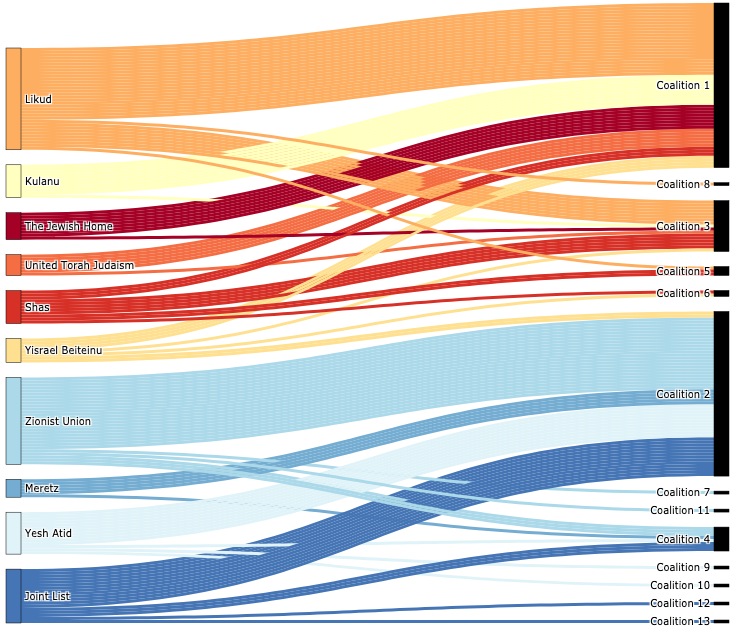
\includegraphics[width=\columnwidth]{pac_friends}
\caption{Coalitions formed by the PAC friends model, compared to party affiliations. Left wing parties are colored with blue hues, right wing red hues, center yellow hues.}
\end{figure}

\begin{table}[h!]
\centering
\begin{tabular}{c|c|c|c|c}
\hline
\multirow{2}{*}{ PAC Model } & \multicolumn{2}{c|}{ No. Coalitions } & \multicolumn{2}{|c}{ Norm Info Dist } \\
& mean & variance & mean & variance \\
\hline
Value Function & 87 & 0 & 0.526 & 0 \\
Friends & 13 & 1.6669 & 0.617 & 0.0003 \\
Selective friends & 20 & 3.3391 & 0.598 & 0.0001 \\
\hline
\end{tabular}
\caption{Each PAC model is implemented using the PAC top covering algorithm; choice set approximation are done with $3/4$ of all bills; the model is executed 50 times on the same Knesset dataset.}
\label{table:pac_models}
\end{table}

\subsection{Comparison Models} \label{subsec:exp_comparison_models}
We want to see how our PAC hedonic game models compare to established models commonly used for partitioning problems.

\paragraph{Clustering: $k$-means}
$k$-means has the advantage of being a general purpose method requiring little hyperparameter tuning. It also runs quickly in practice.
The main drawback of k-means is that it assumes the clusters to be of similar size.
Our ground truth partition by party isn't an extreme case of dissimilar sized clusters; it definitely has some variability\footnote{party size statistics: max=34, min=6, median=11, mean=14.7, stdev=9.6}.

Since $k$-means produces a partition of $k$ clusters by minimizing with-cluster sum-of-squares (WSS), we need to define the distance between points and choose an appropriate $k$ value.
A politician corresponds to a point; each bill is a feature. A politician's ``for'' vote on a bill is assigned value of 1, ``against'' vote assigned value of -1; any other vote value including missing and ``abstained'' is assigned 0.
This simple vote value encoding captures the idea that ``for'' and ``against'' votes are far from each other; anything else is neutral and has equal distance from ``for'' and ``against''.

We ran k-means clustering for $k$ in range $[2, 100]$, and determined the best $k=10$ by plotting cluster size against the corresponding partition's total WSS and picking the point where there is a ``bend'' in the plot – this is known as the elbow method for $k$ selection. The elbow in the plot represents a point where adding one more cluster doesn't bring much improvement to WSS anymore.

One might argue that the average silhouette method provides a quantitative definitive selection of $k$. On our Knesset dataset the average silhouette peaks at $k=2$ and decreases significantly thereafter.

\paragraph{Community Detection: Weighted Stochastic Block Model}
Community detection approach models the dataset as a graph with parliament members as nodes and how frequently a pair of members voted together/differently as edge weights. The stochastic block model assumes that nodes that belong to the same group have the same probability of being connected with other nodes of the network. Using Bayesian inference, it finds a partition that maximizes the likelihood of observed network. It is equivalent to the {\it minimum description length method} where given the same explanatory power, the simplest model is selected. This gives the SBM approach some tolerance for stochastic noise.

We construct the first SBM with only positive edge weights – each edge weight represents the number of times a pair of politicians voted together, either for or against a bill. We model the edge weights using the geometric distribution given the weights are non-negative and discrete values.

The second SBM accounts for instances when a pair of politicians' votes disagreed – edge weight is the difference of the number of times their votes agreed and the number of times their votes disagreed. Since the edge weights can be negative, we model the weights using the normal distribution.

Given that we are analysing an empirical network, there could be more than one fit of the SBM with similar likelihoods of generating the observed network. Therefore instead of finding the maximum, we sample partitions from the posterior distribution, and take the average weighted by posterior probabilities across different model fits. We use the SBM implemented in the graph-tool library, which supports model averaging using an efficient Markov chain Monte Carlo (MCMC) algorithm. This further optimizes the SBM models.

\subsection{Experiment Analysis} \label{subsec:exp_analysis}

One technical note before we delve into analyzing the outcome: due to Knesset members resigning mid term, some Knesset members have only been able to participate in some of the votes, and therefore they will often be clustered separately. Moreover, some government ministers which are also Knesset members have a low rate of participation in the votes, and therefore, once again, their data is sometimes skewed.

\begin{figure}[htb]
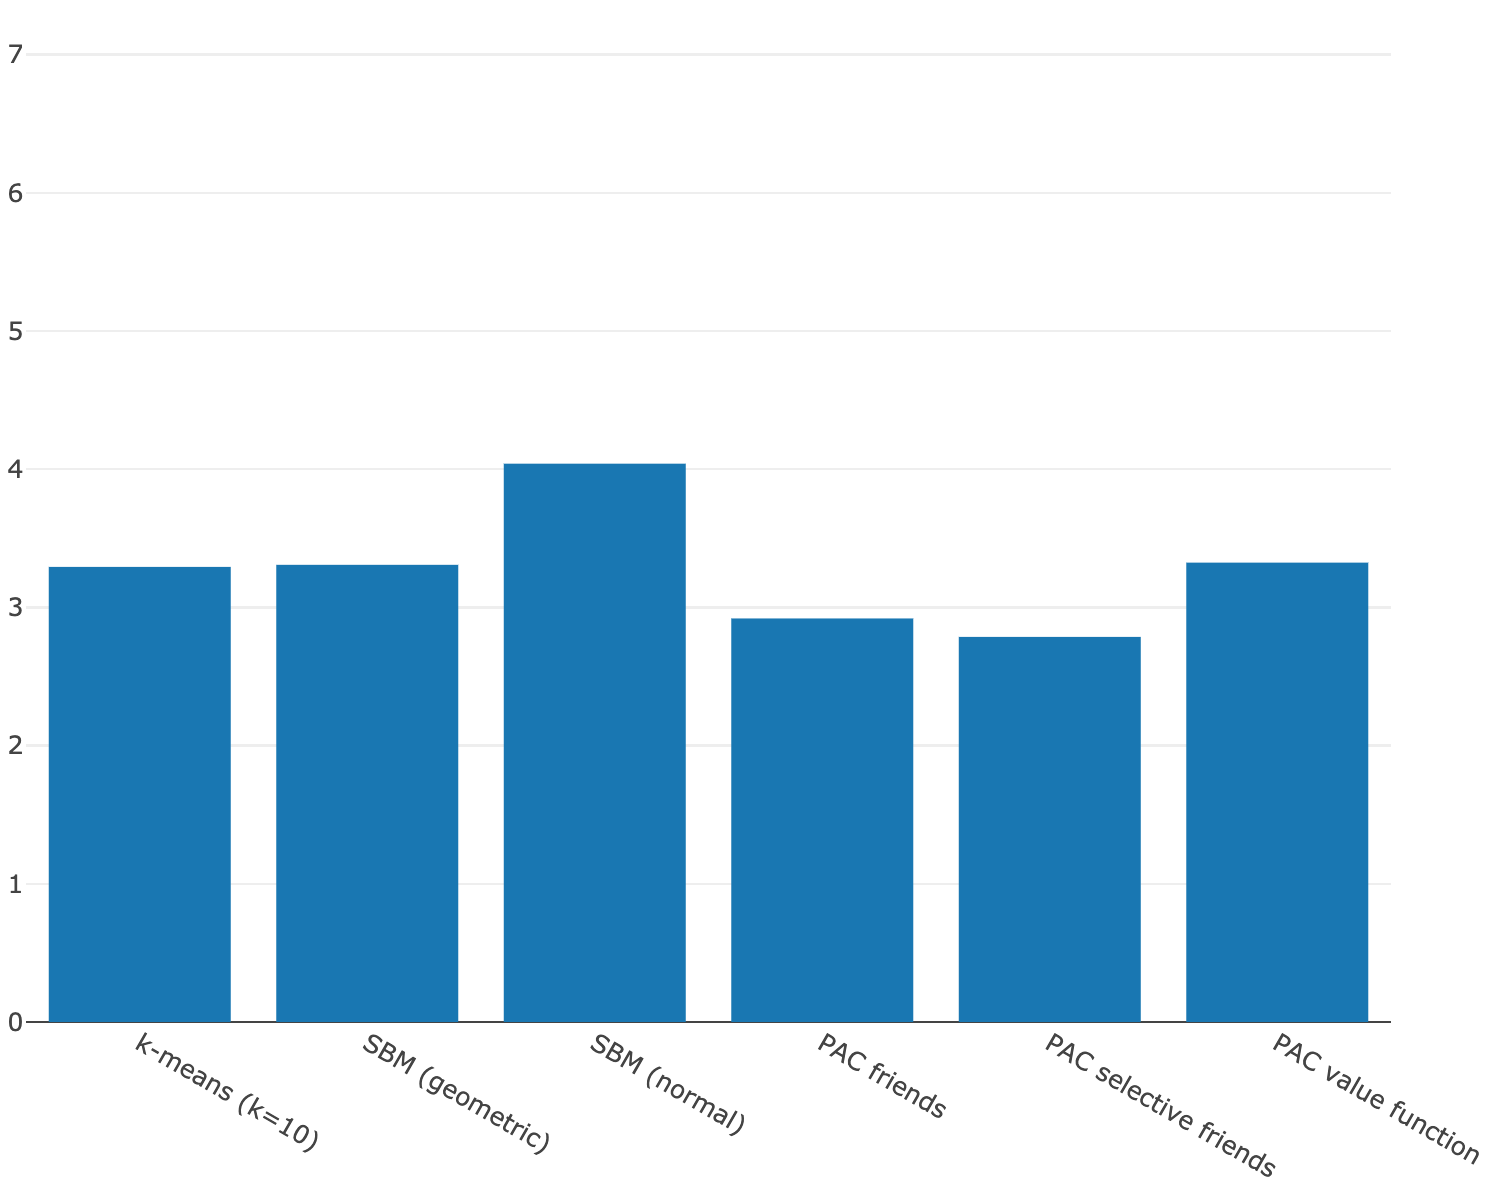
\includegraphics[width=.8\columnwidth]{AAAITemplate/exp_vi.png}
\caption{Variation of Information (VI) between Model Partition and Party Partition --- the lower the better}

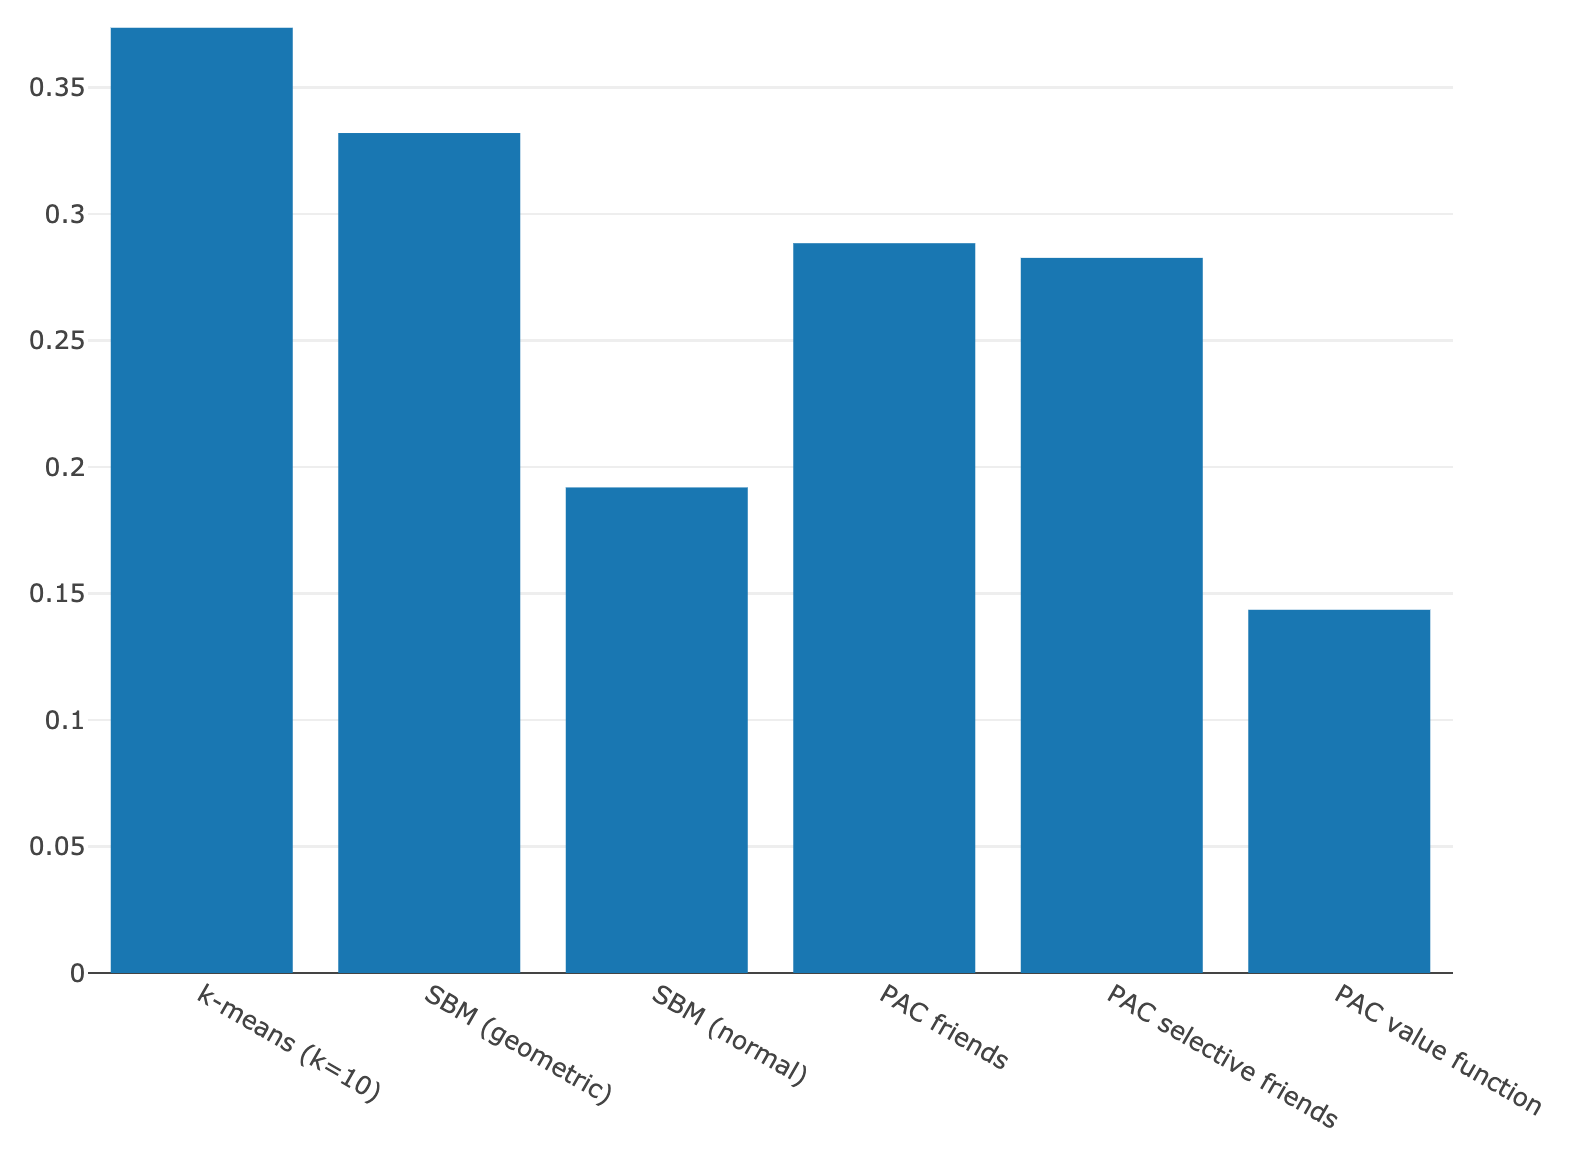
\includegraphics[width=.8\columnwidth]{AAAITemplate/exp_ami.png}
\caption{Adjusted Mutual Information (AMI) between Model Partition and Party Partition --- the higher the better}
\end{figure}

As noted above, the PAC model with the value function produces low quality results (in this case, a grouping of part of the government's coalition, and many singletons, containing only one Knesset member), as well as many of the k-means outcomes and the community models distributions. We shall focus in this comparison on the PAC models with friends and selective friends, the 2-group and 10-group k-means outcomes (selected using the average silhouette method and elbow method, respectively), and the normal and geometric distributions for the community models.

\paragraph{Coherence}
Seeing whether the opposition and government coalition party members were well separated by the different models, resulting in a coherent and logical map.

Under this criterion, the PAC model, particularly with selective friends was the only one which did not include several groups involving many members of different ideological hue. Both the k-means and the community models tended to join together members with fewer votes. However, the PAC selective friends model has only two such coalitions: One involving Knesset member which changed parties (so connecting her with the opposition group makes sense), and the other one creating a single group combining two low-attendance members, one on the right edge of the left wing, and the other, which switched between coalition and opposition.

\paragraph{Overall structure}
Both PAC models and the k-means one were able to figure out that there is a main government group and a main opposition group, to which most of their respective members were attached. This stresses the fact that despite their differences, even the opposition parties, which do not have a centralized binding instructions, still tend to vote together due to their relative ideological cohesion. The community based models, however, did not really pick up on the existence of generally quite coherent group of government and opposition Knesset members.

Most other groups were created based on attendance, with the PAC models more clearly creating a few singleton coalitions for less present members, while clustering ministers, which tend to miss out on votes, together (though in two different coalitions). The k-means clusters tended to remove more ministers from the overall main government group, and divide them into more separate coalitions (this is also true for the community models).

\paragraph{Sub groups}
None of the models was able to differentiate between the subgroups inside parties, apart from identifying a significant change (e.g., a member switches parties). We believe this is more of an indication of the process of ideological coherence happening in Israeli parties. Parties that have been running sharing a similar location on the ideological spectrum and recently join together to run as a single ticket do not have many opportunities to flaunt their differences. Thus, even for a party (such as the Joint List) that did not run together in the following election, it does not seem that their Knesset members voted differently. Indeed, several of their Knesset members, despite being from different parties (and running separately in the following election) have not been assigned to different coalitions by any model, or even any run of the PAC models. As noted above, we believe this tells us a meaningful statement on the real, day to day, ideological difference between them, and is not a failure of the algorithms.

\section{Conclusions and Future Work} \label{sec:conclusion}
Our work demonstrates the viability and power of PAC top responsive game model on real-world data through a case study on the Israeli Parliament. A natural next step is to apply our selective friends model on other parliaments, such as the Netherlands which also has a coalition government; the United States congress could be interesting as we could test if the model reveals any regional effect. Another research direction is to extend existing stable solution discovery algorithms, such as the bottom avoiding algorithm by \citename{SuSu10}, to discover PAC stable partitions and compare with the selective friends model.

\bibliography{references}
\bibliographystyle{aaai}

\end{document}

